\documentclass[10pt,a4paper]{article}

\usepackage[utf8]{inputenc}
\usepackage[T1]{fontenc}
\usepackage{helvet}
\renewcommand{\familydefault}{\sfdefault}
\usepackage[top=15mm,bottom=17mm,left=15mm,right=15mm]{geometry}
\usepackage{graphicx}
\usepackage{amsmath}
\usepackage{sansmath}
\sansmath
\usepackage{booktabs}
\usepackage{xcolor}
\usepackage{hyperref}
\hypersetup{
  colorlinks=true,
  linkcolor=blue!60!black,
  citecolor=green!50!black,
  urlcolor=blue!70!black,
  pdftitle={alight: scriptable solid-propellant grain burnback},
  pdfauthor={Jake Boening}
}
\usepackage{cleveref}
\usepackage{float}
\usepackage{siunitx}
\sisetup{mode=text}
\usepackage{enumitem}
\usepackage{fancyhdr}
\usepackage{lastpage}
\usepackage{titlesec}
\titleformat{\section}{\normalsize\bfseries}{\thesection.}{0.5em}{}
\titlespacing*{\section}{0pt}{7pt plus 2pt minus 2pt}{3pt}
\graphicspath{{../fig/}}

\setlength{\footskip}{22pt}
\setlength{\headheight}{12pt}
\pagestyle{fancy}
\fancyhf{}
\renewcommand{\headrulewidth}{0pt}
\renewcommand{\footrulewidth}{0.4pt}
\fancyfoot[L]{\small alight: \url{https://github.com/jakeboening/alight}}
\fancyfoot[R]{\small Page \thepage\ of \pageref{LastPage}}

\makeatletter
\renewcommand{\maketitle}{%
  \noindent
  \begin{minipage}{\textwidth}
    \centering
    {\large\bfseries \@title}\\[2pt]
    {\normalsize \@author}
  \end{minipage}
  \vspace{3pt}
  \hrule
  \vspace{6pt}
}
\makeatother

\title{alight: Scriptable Solid-Propellant Grain Burnback, Validated Against Closed Forms and a Published Motor}
\author{Jake Boening --- October 2026}

\newcommand{\inch}{\,in}

\begin{document}
\maketitle

\section{Introduction}

A solid rocket motor's pressure and thrust follow the area of its burning surface, and that area
changes as the grain burns back. Computing it for a three-dimensional grain such as a finocyl is
the job of a burnback code. \textbf{alight} is a fork of the open-source burnback-3d
solver~\cite{burnback3d} that makes that computation scriptable end to end:

\begin{itemize}[leftmargin=1.4em,itemsep=0pt,topsep=1pt]
\item \textbf{A command line for the solver.} burnback-3d is a Qt desktop application; mesh import,
  boundary conditions, the run and the export are done by hand. \texttt{alight} runs the same solver
  kernels from a command line, with no Qt and no display, on Linux, Windows and macOS.
\item \textbf{A pipeline around it.} A grain defined by a few numbers is turned into CAD
  (build123d), meshed (Gmsh), solved (\texttt{alight}), reduced to burn area against web, corrected
  for mesh error, and passed to a lumped chamber model for pressure and thrust.
\item \textbf{Checks that can be re-run.} Closed-form grains, a mesh sensitivity study, an
  independent fast-marching solution and a published motor are scripts in the repository.
\end{itemize}

The motivation is control by a language model. An LLM agent cannot reliably click through a GUI or
judge a contour plot, but it can write a grain as numbers, run a command, read a CSV and compare it
with a formula. Every stage here takes text and returns text, none of them prompts, and the checks
that say whether an answer is right are themselves commands. The worked example and this report
were produced that way.

\section{Method}

\textbf{Burn-time field.} With a burn rate that is uniform over the surface, the flame reaches a
point $\mathbf{x}$ of the propellant after burning a web $u(\mathbf{x})$ that satisfies the eikonal
equation
\begin{equation}
  |\nabla u| = 1, \qquad u = 0 \text{ on the initial burning surface}.
\end{equation}
burnback-3d reaches this field on a tetrahedral mesh by marching
$\partial u/\partial\tau = 1 - |\nabla u| + \varepsilon\,D(u)$ in pseudo-time $\tau$ to a steady
state, where $D$ is a diffusive term that keeps the scheme stable. \texttt{alight} runs these
kernels unchanged. Boundary types are the solver's own: \emph{inlet} for the initial burning
surface, \emph{outlet} for the case wall and inhibited faces, \emph{symmetry} for the cut planes of
the smallest repeating wedge, which is all that is meshed.

\textbf{Burn area.} The burning surface at web $w$ is the iso-surface $u = w$. Its area $A(w)$ is
summed over the mesh by marching tetrahedra, exactly for the piecewise-linear field, and multiplied
by the number of wedges.

\textbf{Mesh error and its removal.} The diffusive term makes the scheme first-order accurate: the
computed surface lags the true one by an amount proportional to the element size $h$, more where
the front is strongly curved. On a practical mesh this shifts $A(w)$ by a few percent
(\cref{sec:sensitivity}). Because the error is so nearly linear in $h$, two meshes suffice to
remove its leading term by Richardson extrapolation. Extrapolating $A$ at fixed $w$ would smear
every kink of the curve, since the two meshes place a kink at different webs. The pipeline instead
extrapolates the web at a fixed fraction $f$ of propellant burned,
\begin{equation}
  w_0(f) = \frac{r\,w_{h/r}(f) - w_h(f)}{r - 1}, \qquad r = h_\text{coarse}/h_\text{fine},
\end{equation}
and differentiates the result, $A = V_p\,\mathrm{d}f/\mathrm{d}w_0$, with $V_p$ the meshed propellant
volume. Kinks stay sharp and the propellant mass is conserved exactly.

\textbf{Ballistics.} A lumped chamber follows
$\mathrm{d}P/\mathrm{d}t = (RT_c/V)\,[(\rho_p - \rho_g)A\,\dot r - P A_t/c^*]$ with
$\dot r = aP^n$, free volume $V(w)$ from the burn table, and thrust $F = C_F P A_t$ for an ideal
nozzle. Erosive burning, axial pressure drop, throat erosion and the ignition transient are not
modelled.

\section{Validation against closed forms}
\label{sec:closed}

Three grain families with closed-form burn area were run through the whole pipeline, each swept
over its geometry (15 cases; case diameter \SI{10}{in}):

\begin{itemize}[leftmargin=1.4em,itemsep=0pt,topsep=1pt]
\item \textbf{Tube}, ends inhibited: $A = 2\pi(r_p + w)L$. Port-to-case ratio 0.2 to 0.8.
\item \textbf{BATES}, both ends burning:
  $A = 2\pi(r_p + w)(L - 2w) + 2\pi\,[R^2 - (r_p + w)^2]$. Length-to-diameter ratio 0.5 to 1.5.
\item \textbf{Star}, ends inhibited: the classical two-phase perimeter of a star with flat flanks
  and a filleted tip. Number of points 5 to 8, angular fraction 0.5 to 0.9, point angle
  \SI{60}{\degree} to \SI{100}{\degree}. The formulas were first checked against a numerical
  offset of the star outline (within 0.06\,\%) and against the CAD volume (to six digits).
\end{itemize}

\Cref{tab:closed} gives the difference from the closed form over the first 95\,\% of the web. The
last 5\,\% is excluded because the burn area is discontinuous at burnout, which any mesh spreads
over about one element; the burnout web is compared instead. \Cref{fig:tube,fig:bates,fig:star}
show the curves.

\begin{table}[H]
\centering\small
\caption{Extrapolated burn area against the closed form, ignition to 95\,\% of the web. ``Fine
mesh'' is the same comparison for the finer of the two meshes without extrapolation.}
\label{tab:closed}
\begin{tabular}{llrrrrr}
\toprule
Family & Case & Tetrahedra & Max (\%) & RMS (\%) & Fine mesh RMS (\%) & Burnout web (\%) \\
\midrule
Tube & port / case = 0.2 & 404\,497 & 0.16 & 0.14 & 0.21 & +0.04 \\
Tube & port / case = 0.4 & 353\,854 & 0.15 & 0.14 & 0.09 & +0.03 \\
Tube & port / case = 0.6 & 270\,593 & 0.14 & 0.13 & 0.05 & +0.02 \\
Tube & port / case = 0.8 & 153\,053 & 0.14 & 0.14 & 0.02 & +0.00 \\
BATES & L / D = 0.5 & 439\,570 & 0.79 & 0.14 & 0.36 & +0.57 \\
BATES & L / D = 1 & 875\,969 & 0.18 & 0.09 & 0.30 & -0.01 \\
BATES & L / D = 1.5 & 1\,311\,133 & 0.23 & 0.12 & 0.27 & -0.01 \\
Star & N = 5 & 730\,709 & 0.20 & 0.13 & 0.40 & -- \\
Star & N = 6 & 600\,182 & 0.12 & 0.04 & 0.39 & -- \\
Star & N = 7 & 488\,962 & 0.16 & 0.07 & 0.40 & -- \\
Star & N = 8 & 423\,514 & 0.27 & 0.14 & 0.41 & -- \\
Star & angular fraction 0.5 & 547\,546 & 0.25 & 0.19 & 0.30 & -- \\
Star & angular fraction 0.9 & 678\,836 & 0.19 & 0.11 & 0.48 & -- \\
Star & point angle 60\si{\degree} & 616\,484 & 0.26 & 0.14 & 0.30 & -- \\
Star & point angle 100\si{\degree} & 563\,847 & 0.26 & 0.20 & 0.52 & -- \\
\bottomrule
\end{tabular}
\end{table}

The extrapolated burn area is within 0.27\,\% of the closed form in every case but one, and
within 0.20\,\% RMS in all of them. The exception is the shortest BATES grain, whose two
end faces meet at burnout: its largest difference, 0.79\,\%, is in the last few percent of
the compared range, next to that discontinuity. The agreement is not exact. A residual of about
0.1\,\% remains after extrapolation, and for the thin-web tube it is larger than the already small
error of the fine mesh alone.

\begin{figure}[H]
\centering
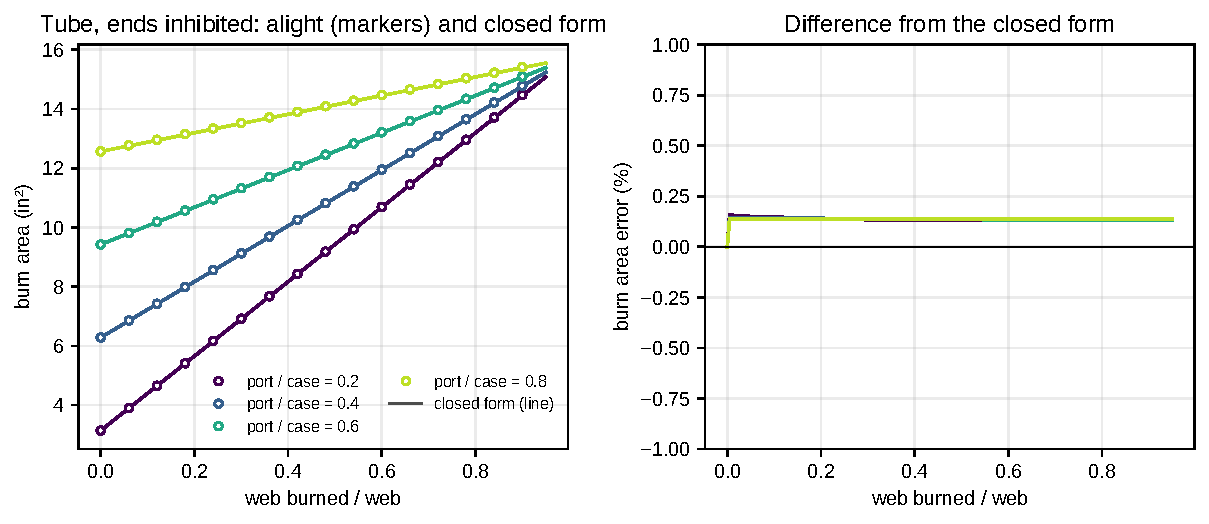
\includegraphics[width=0.86\textwidth]{validation_tube.pdf}
\caption{Tube grains: burn area and its difference from the closed form.}
\label{fig:tube}
\end{figure}
\begin{figure}[H]
\centering
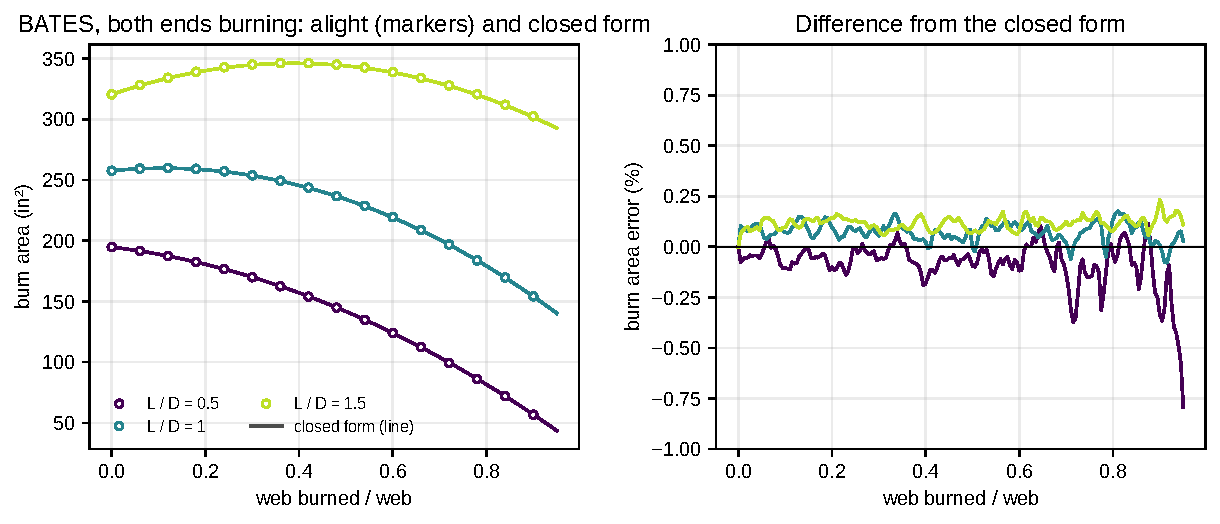
\includegraphics[width=0.86\textwidth]{validation_bates.pdf}
\caption{BATES grains.}
\label{fig:bates}
\end{figure}
\begin{figure}[H]
\centering
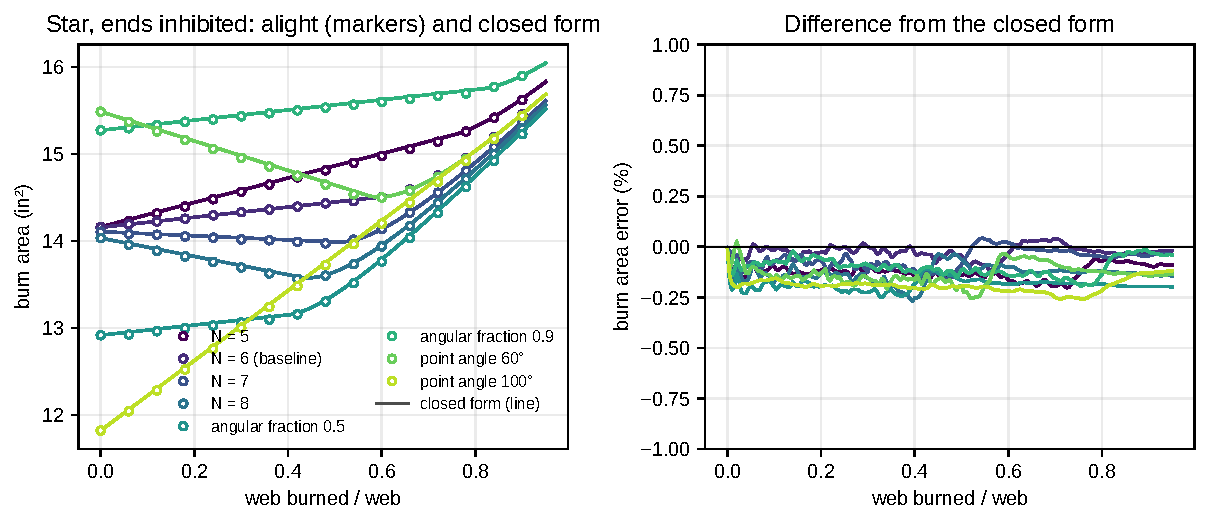
\includegraphics[width=0.86\textwidth]{validation_star.pdf}
\caption{Star grains. The comparison ends where the star's arcs reach the case; the slivers that
burn after that have no simple closed form.}
\label{fig:star}
\end{figure}

\section{Mesh sensitivity on a finocyl grain}
\label{sec:sensitivity}

The worked example is a finocyl grain: \SI{10}{in} outer diameter, \SI{4}{in} port, \SI{60}{in}
long, six \SI{1}{in} fins with semicircular tips reaching a \SI{4}{in} radius over the aft
\SI{20}{in}, case-bonded with both ends inhibited. It was solved on seven meshes, from
\SI{0.4}{in} to \SI{0.05}{in} elements (24 thousand to 9.8 million tetrahedra in the
\SI{30}{\degree} wedge), and each neighbouring pair was extrapolated. The propellant is an
aluminized AP/HTPB composite with representative values ($\rho = \SI{1800}{kg/m^3}$,
$\dot r = \SI{0.35}{in/s}$ at \SI{1000}{psi}, $n = 0.35$, $c^* = \SI{1580}{m/s}$,
$\gamma = 1.14$), and the throat (\SI{2.70}{in}) is sized for a \SI{1000}{psi} peak.

\begin{figure}[H]
\centering
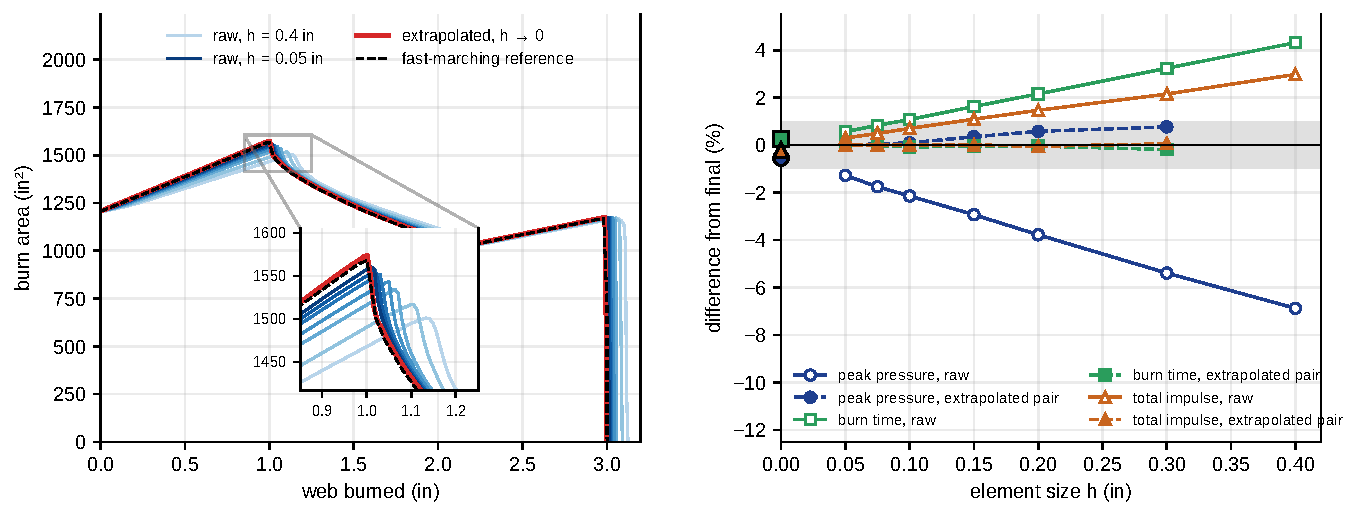
\includegraphics[width=0.95\textwidth]{finocyl_sensitivity.pdf}
\caption{Left: burn area for the seven meshes, the extrapolated result and the fast-marching
reference. Right: peak pressure, burn time and total impulse against element size, as difference
from the final result; symbols at $h = 0$ are the reference, the band is $\pm1\,\%$.}
\label{fig:sens}
\end{figure}

\begin{itemize}[leftmargin=1.4em,itemsep=0pt,topsep=1pt]
\item \textbf{Raw results depend on the mesh.} Peak pressure spans 5.6\,\% over the seven meshes
  and still moves 0.49\,\% at the last refinement. The error falls linearly with $h$: fitted
  orders are 0.81 for peak pressure, 0.98 for burn time and 1.04 for burnout web.
\item \textbf{Extrapolated results do not.} For every pair from 0.2/0.15\inch\ down, peak pressure,
  burn time and total impulse stay within 0.35\,\%; the last two pairs differ by at most 0.05\,\%.
\item \textbf{An independent method agrees.} The distance from the initial port was computed on a
  \SI{0.035}{in} Cartesian grid by fast marching (scikit-fmm), with burn area from marching cubes
  (scikit-image). The final result differs from it by 0.55\,\% in peak pressure, 0.26\,\% in burn
  time and 0.22\,\% in total impulse. The closed-form distance on the same grid agrees with the
  fast-marching one within 0.16\,\%.
\item \textbf{Solver settings.} The CFL number and the convergence tolerance do not change the
  converged field. The diffusive weight changes the raw result by about 6\,\% but the extrapolated
  one by about 1\,\%; weights below about 0.75 diverge.
\end{itemize}

\begin{figure}[H]
\centering
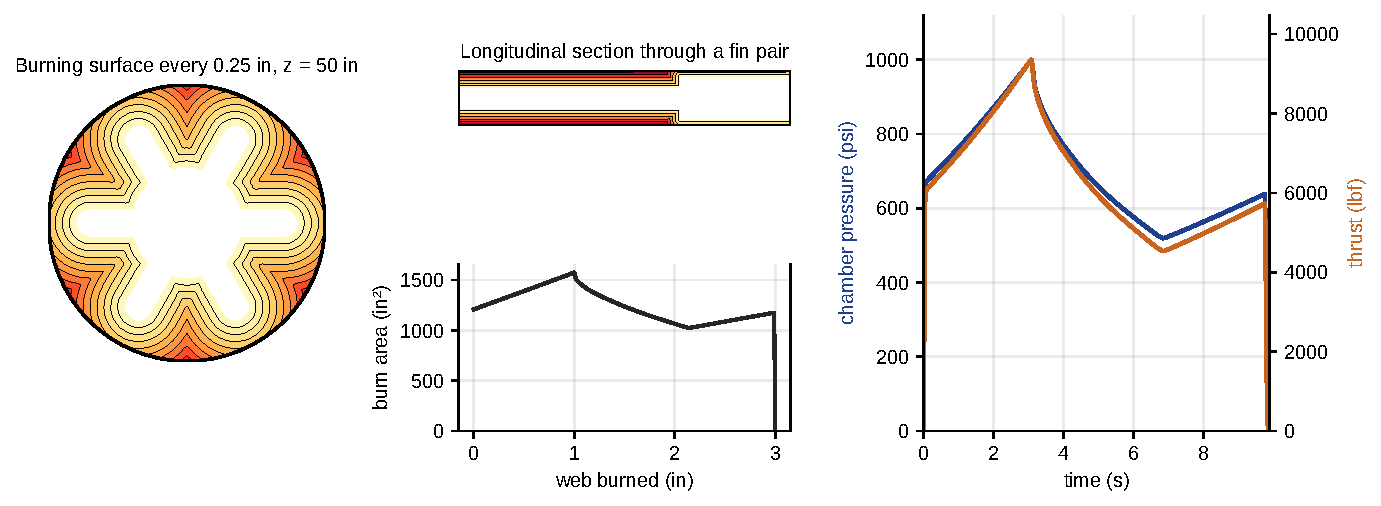
\includegraphics[width=0.95\textwidth]{finocyl_results.pdf}
\caption{Finocyl example: burning surfaces, burn area, chamber pressure and thrust. Burn area peaks
when the fin tips reach the case (web \SI{1.00}{in}), falls as the slots burn out, and rises again
in the plain port until burnout (web \SI{3.00}{in}). Peak thrust \SI{9355}{lbf}, burn time
\SI{9.82}{s}, total impulse \SI{61559}{lbf.s}, propellant mass \SI{110}{kg}.}
\label{fig:finocyl}
\end{figure}

\section{Comparison with a published motor}
\label{sec:nawc}

NAWC tactical motor no.~6 is a reduced-smoke motor fired at China Lake~\cite{blomshield} and
simulated by Willcox et al.~\cite{willcox} with the Rocgrain three-dimensional burnback code. Its
grain (\SI{5}{in} diameter, \SI{69.4}{in} long) has a cylindrical bore at the head end that changes
over tapered transitions into a six-slot star. Figure~7 of \cite{willcox} dimensions it at seven
stations, which were entered as a station-defined grain; the \SI{0.213}{in} rounding where a slot
meets the bore was left out, and the aft face was taken as burning because only the forward face is
marked inhibited. The propellant is from Table~3 of \cite{blomshield}: \SI{1.80}{g/cm^3},
\SI{0.678}{cm/s} at \SI{6.9}{MPa}, exponent 0.36. Neither source states $c^*$; it was derived from
the tabulated chamber speed of sound (\SI{1083}{m/s}) with an assumed $\gamma = 1.2$, giving
1524\,m/s. The throat is \SI{1.84}{in}.

\Cref{fig:nawc} compares chamber pressure with Figure~10 of \cite{willcox}, read from the paper's
vector graphics. The like-for-like reference is the paper's 0-D simulation with the strand burn
rate, which makes the same modelling assumptions as this pipeline.

\begin{figure}[H]
\centering
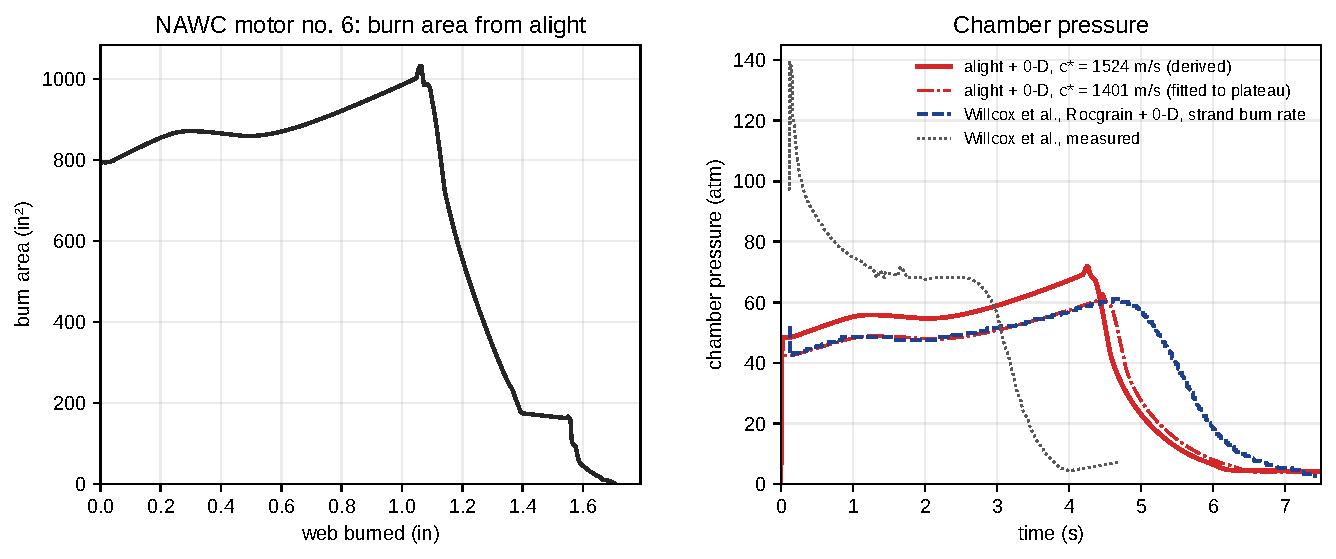
\includegraphics[width=0.95\textwidth]{nawc_motor6.pdf}
\caption{NAWC motor no.~6. Left: burn area from alight. Right: chamber pressure from alight with
0-D ballistics, the published 0-D simulation with the strand burn rate, and the measured trace.}
\label{fig:nawc}
\end{figure}

With the propellant data as published and the derived $c^*$, the predicted trace has the shape of the published simulation but sits 14\,\% higher over the plateau (0.3 to \SI{3}{s}) and peaks 8\,\% earlier. That is the size of offset an uncertain $c^*$ produces: pressure scales as $(c^*)^{1/(1-n)}$. Fitting that one constant to the published plateau gives $c^* = 1401$\,m/s. With it, the plateau agrees within 1.4\,\% RMS, the peak pressure within 3\,\% (63.0 against 61.1\,atm) and the time of the peak within 3\,\% (4.46 against 4.60\,s). The progressive rise to the peak, which is set by the slots burning outward, is reproduced. The tail-off is not: alight's pressure falls through half its peak at 4.9\,s, the published simulation at 5.7\,s. The cause was not isolated; candidates are the simplifications listed above and differences in how the two 0-D models treat the slivers. The measured trace is higher and much shorter than both simulations (plateau near 68\,atm, burnout near 3.3\,s). Willcox et al. attribute that to erosive and dynamic burning and reproduce it only with a modified burn rate, so the measurement tests the ballistic model, not the burnback.

\section{Portability}

\texttt{alight} is plain C++17 with one header-only dependency and builds with CMake. It was
cross-compiled for Windows and run under Wine~10: on a 6,292-node mesh the Windows and Linux
executables converged in the same number of iterations and their burn-time fields agree to
$1.4\times10^{-14}$\,mm. The pipeline's test suite (CAD, mesh, solver, burn area) also passes with the Windows executable substituted for the Linux one. A continuous-integration job builds \texttt{alight} natively on Linux, Windows and macOS and runs the pipeline tests on Linux and Windows. The Python pipeline uses numpy, scipy, matplotlib,
build123d and gmsh, all of which publish Windows wheels, and calls nothing platform-specific.

\section{Summary and limits}

\begin{itemize}[leftmargin=1.4em,itemsep=0pt,topsep=1pt]
\item The burnback-3d solver, run from a command line and wrapped in a scripted pipeline, reproduces
  closed-form burn area within about 0.27\,\% for tube, BATES and star grains over 15
  geometries.
\item Its raw results are first-order in element size and shift by several percent between
  practical meshes. Extrapolating two meshes at fixed fraction burned removes that: results then
  agree within 0.35\,\% across mesh pairs and within 0.6\,\% of an independent fast-marching
  solution.
\item For NAWC motor no.~6, with $c^*$ fitted as the one free constant, the pressure plateau agrees with the published three-dimensional burnback simulation within 1.4\,\% RMS and the peak within 3\,\% in level and time; the tail-off is 14\,\% shorter. Without the fit the pressure is 14\,\% higher.
\item Limits: uniform burn rate over the surface at each instant, so no erosive burning or axial
  pressure drop; no throat erosion or ignition transient; propellant values in the worked example
  are representative, not a qualified formulation. No Solid Performance Program (SPP) case could be
  reproduced: SPP is export-controlled, and its public manual~\cite{spp} gives pressure traces for
  its validation motors but not their grain inputs.
\end{itemize}

\begin{thebibliography}{9}\small
\bibitem{burnback3d} iff, \emph{burnback-3d}, \url{https://codeberg.org/iff/burnback-3d}.
\bibitem{willcox} M.~A. Willcox, M.~Q. Brewster, K.~C. Tang, D.~S. Stewart and I.~Kuznetsov,
  ``Solid Rocket Motor Internal Ballistics Simulation Using Three-Dimensional Grain Burnback,''
  \emph{Journal of Propulsion and Power}, Vol.~23, No.~3, 2007, pp.~575--584.
  doi:\href{https://doi.org/10.2514/1.22971}{10.2514/1.22971}.
\bibitem{blomshield} F.~S. Blomshield, \emph{Pulsed Motor Firings}, NAWCWD TP~8444, Naval Air
  Warfare Center Weapons Division, China Lake, CA, 2000. DTIC ADA382239.
\bibitem{spp} D.~E. Coats et al., \emph{A Computer Program for the Prediction of Solid Propellant
  Rocket Motor Performance}, AFRPL-TR-75-36, Vols.~I--II, 1975. DTIC ADA015140, ADA015141.
\end{thebibliography}

\end{document}
